\setcounter{figure}{2}
\begin{figure}[H]
\centering
\par\smallskip\textbf{Panel 3; provisional numerical counterpart: partially reproduced}\par
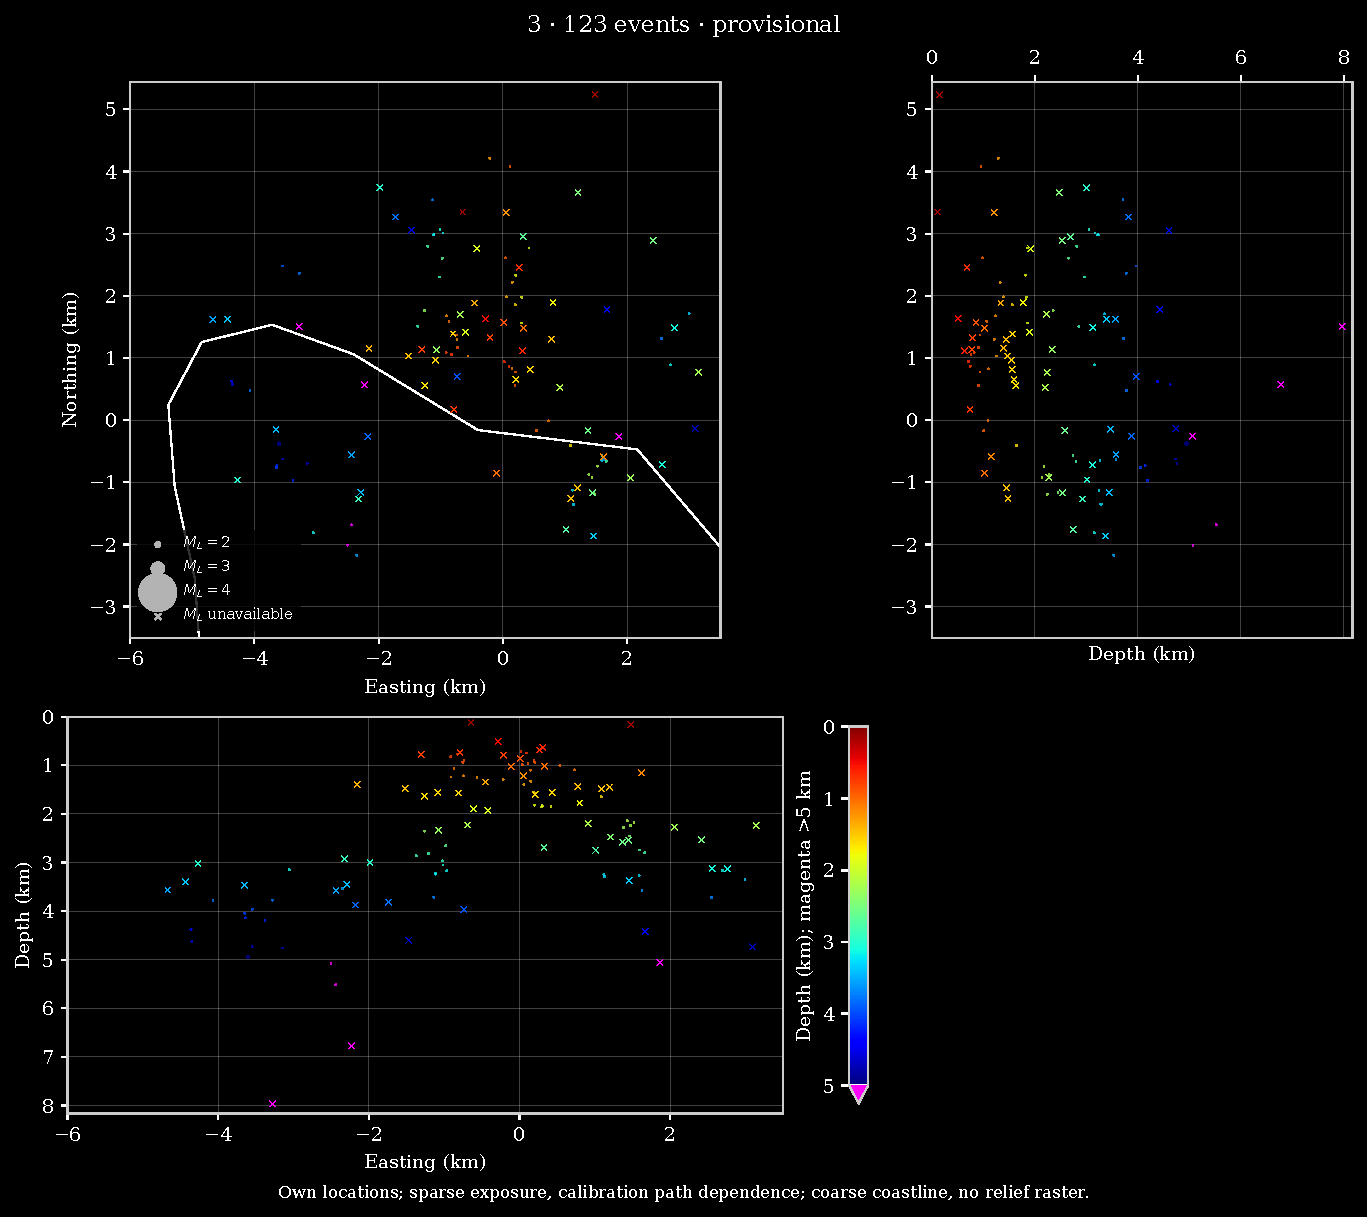
\includegraphics[width=.94\linewidth,height=0.310\textheight,keepaspectratio]{figures/figure_3_provisional.pdf}
\par\smallskip\textbf{Panel Latest extended cohort: independently rerun, provisional: partially reproduced}\par
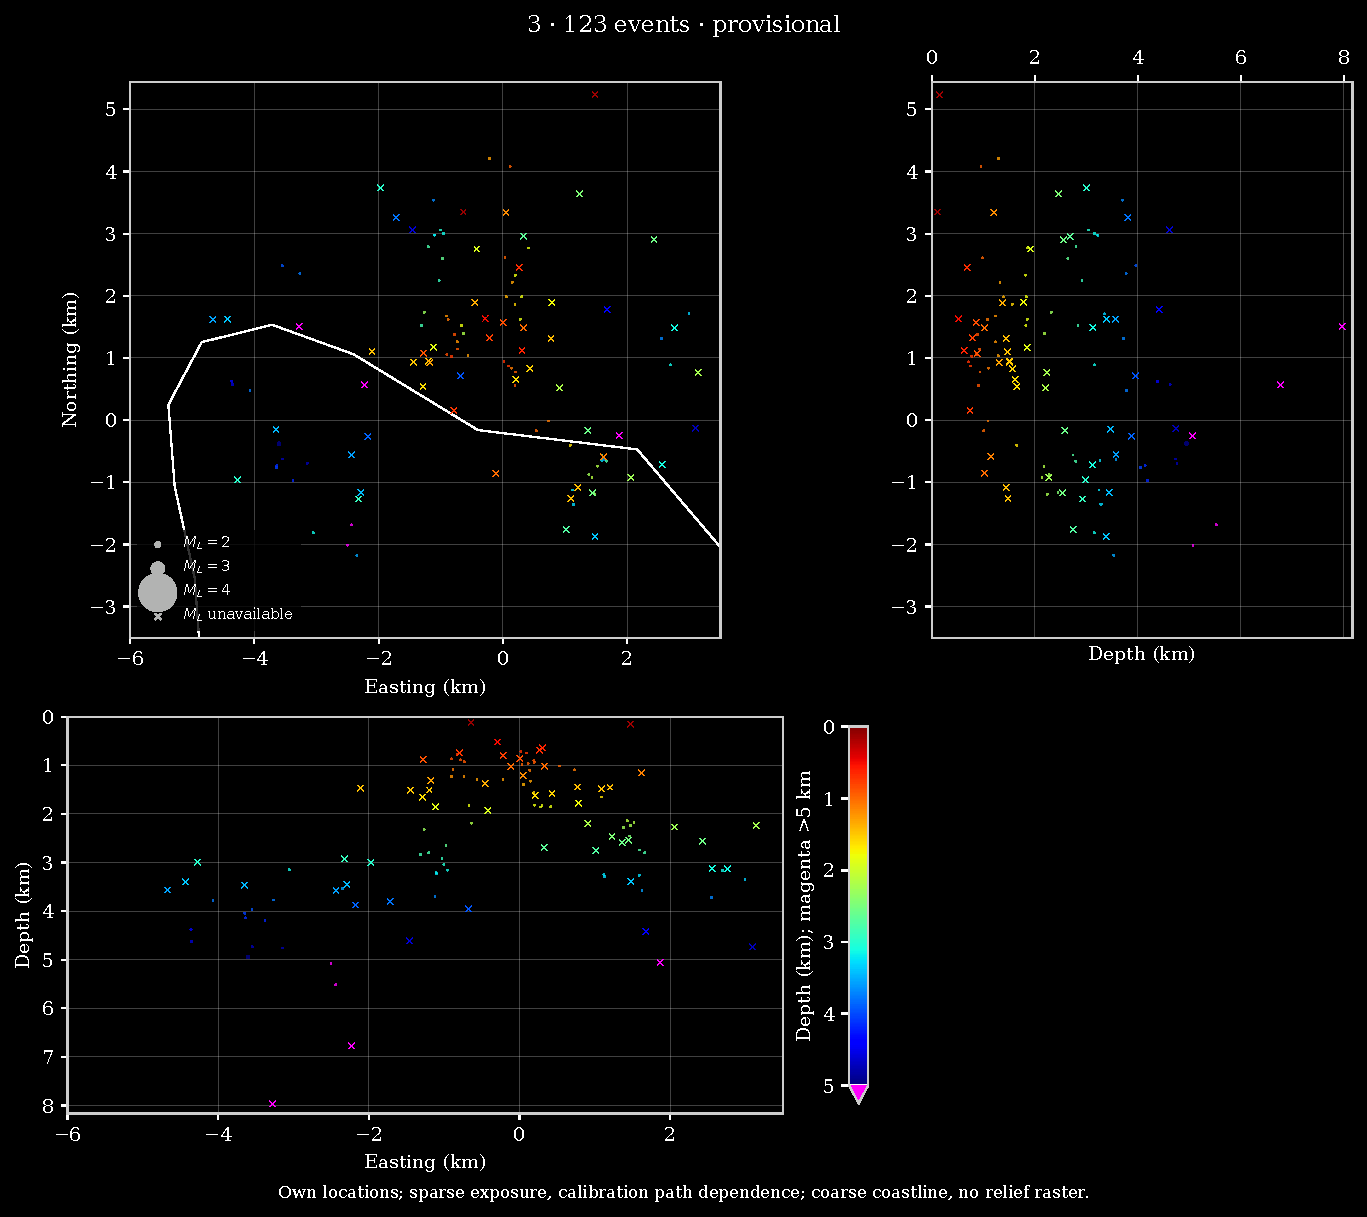
\includegraphics[width=.94\linewidth,height=0.310\textheight,keepaspectratio]{figures/figure_3_extension.pdf}
\caption{Spatial distribution of seismicity. 123 independently relocated trial events, 0.111--7.965 km depth. Own relative magnitudes set sizes where available; crosses mark missing magnitudes. This scattered subset does not establish the published ring or its depth limit. Provisional independent observations and processing; sparse coverage, unreviewed phases, calibration path sensitivity. Not established fault geometry or exact reproduction. The additional extended-cohort view uses separately numbered, independently rerun results. Magnitudes and SVD uncertainties were not inherited by integer event ID.}
\label{publication:3}
\end{figure}
